\documentclass[english,finnish]{beamer}
\usepackage[utf8]{inputenc}
%\usepackage[T1]{fontenc}
\usepackage[finnish]{babel}
\usepackage{fancyvrb}
\RecustomVerbatimEnvironment{verbatim}{Verbatim}{}
\usetheme{Warsaw}
\usecolortheme{orchid}
\title[FIPUG 2015-03-19]{Kolme pientä PostGIS-esimerkkiä}
\author{Jonne Savolainen \and Janne Upla}
\date{19. maaliskuuta 2015}
\begin{document}

\begin{frame}
\titlepage
\end{frame}

\begin{frame}{PostGIS lyhyesti}
  \begin{itemize}
  \item
    PostGIS on PostgreSQL:n laajennosrajapintaa käyttävä lisäosa, joka
    toteuttaa Simple Features Specification -määrittelyn
    (\url{http://www.opengeospatial.org/standards/})
  \item Projekti perustettu vuonna 2001
  \item Tukee tasogeometrioita (GEOMETRY), spheroidigeometrioita
    (GEOGRAPHY) ja rasteritiiliä (RASTER)
  \item Kevyt arkkitehtuuri, satoja funktioita
    \item Perusteellinen esittely:
      \url{http://workshops.boundlessgeo.com/postgis-intro/}
\end{itemize}
\end{frame}

\begin{frame}{Esimerkki 1: Postinumeroaineiston yleistäminen}
  Yleistysprosessi (Janne Upla)
  \begin{itemize}
  \item Perustetaan PostGIS-kanta \texttt{postgis\_topology}-laajennoksella
  \item Ladataan taulu Tilastokeskuksen WFS-palvelusta tietokantaan
    ogr2ogr-työkalulla (\url{http://www.gdal.org/})
  \item Muodostetaan topologinen malli
  \item Yleistetään rajaviivageometrioita topologisen mallin avulla
  \item Vertailun vuoksi yleistetään polygonit ilman topologista mallia
\end{itemize}
\end{frame}



\begin{frame}[fragile=singleslide]\frametitle{Esimerkki 1: PostGIS-kannan perustaminen}
Luodaan ensin tyhjä Postgres-kanta (versio $\ge$ 9.1), omistaja fipug.
\begin{verbatim}
$ createdb -U postgres -O fipug fipug

$ psql -U postgres -d fipug
CREATE EXTENSION postgis;
CREATE EXTENSION postgis_topology;
GRANT ALL ON SCHEMA topology TO fipug;
GRANT ALL ON ALL TABLES IN SCHEMA topology TO fipug;
GRANT ALL ON ALL SEQUENCES IN SCHEMA topology TO fipug;

CREATE SCHEMA statfi;

ALTER DATABASE fipug
SET search_path = statfi, public, topology, pno_meri_topo;
\end{verbatim}
\end{frame}

\begin{frame}[fragile=singleslide]\frametitle{Esimerkki 1: Ladataan
    aineisto tietokantaan}
\begin{verbatim}[fontsize=\footnotesize]
$ ogr2ogr -overwrite -f PostgreSQL\
  PG:"user=fipug host=localhost port=5433 dbname=fipug"\
  WFS:http://geo.stat.fi/geoserver/postialue/postialue:pno_meri/wfs\
  -nln pno_meri postialue:pno_meri

-- Tarkistetaan, että tulos on järkevä.
SELECT sum(ST_Area(wkb_geometry)) / 1000000.0 AS km2
FROM statfi.pno_meri;
       km2        
------------------
 390815.261762989
(1 row)
\end{verbatim}
\end{frame}

\begin{frame}[fragile=singleslide]\frametitle{Esimerkki 1: Topologisen mallin luominen}
\begin{verbatim}
SELECT CreateTopology('pno_meri_topo', 3067);
 createtopology 
----------------
              1
(1 row)

SELECT AddTopoGeometryColumn('pno_meri_topo',
    'statfi', 'pno_meri', 'topogeom', 'MULTIPOLYGON');
 addtopogeometrycolumn 
-----------------------
                     1
(1 row)

SET client_min_messages TO WARNING;
UPDATE statfi.pno_meri
SET topogeom = toTopoGeom(wkb_geometry,'pno_meri_topo',1);
\end{verbatim}
\end{frame}

\begin{frame}[fragile=singleslide]\frametitle{Esimerkki 1: Yleistäminen}
\begin{verbatim}
-- Ei-topologinen yleistys
ALTER TABLE statfi.pno_meri
  ADD COLUMN geom_bork geometry(Multipolygon,3067);
UPDATE statfi.pno_meri
  SET geom_bork = ST_Multi(
      ST_SimplifyPreserveTopology(wkb_geometry, 500)
      );

-- Topologinen yleistys
ALTER TABLE statfi.pno_meri
  ADD COLUMN geom_simp geometry(Multipolygon,3067);
UPDATE statfi.pno_meri
  SET geom_simp = ST_Simplify(topogeom, 500);
\end{verbatim}
\end{frame}

\begin{frame}[fragile=singleslide]\frametitle{Esimerkki 1: Alkuperäiset alueet (wkb\_geometry)}
\begin{figure}[h]
\begin{center}
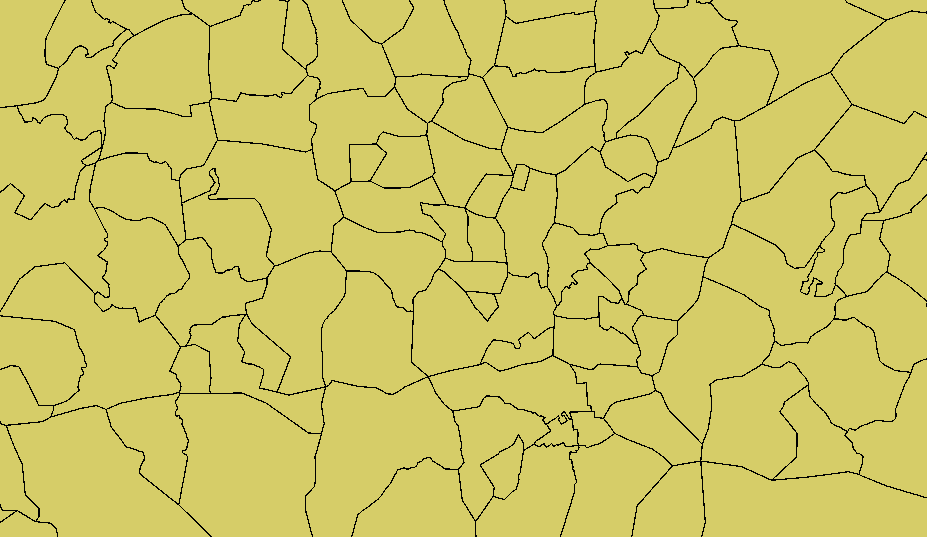
\includegraphics[width=0.90\textwidth]{pnro_base.png}
\caption{Alkuperäiset postinumeroalueet ilman yleistystä.}
\label{kuva1}
\end{center}
\end{figure}
\end{frame}

\begin{frame}[fragile=singleslide]\frametitle{Esimerkki 1: Ei-topologinen yleistys (geom\_bork)}
\begin{figure}[h]
\begin{center}
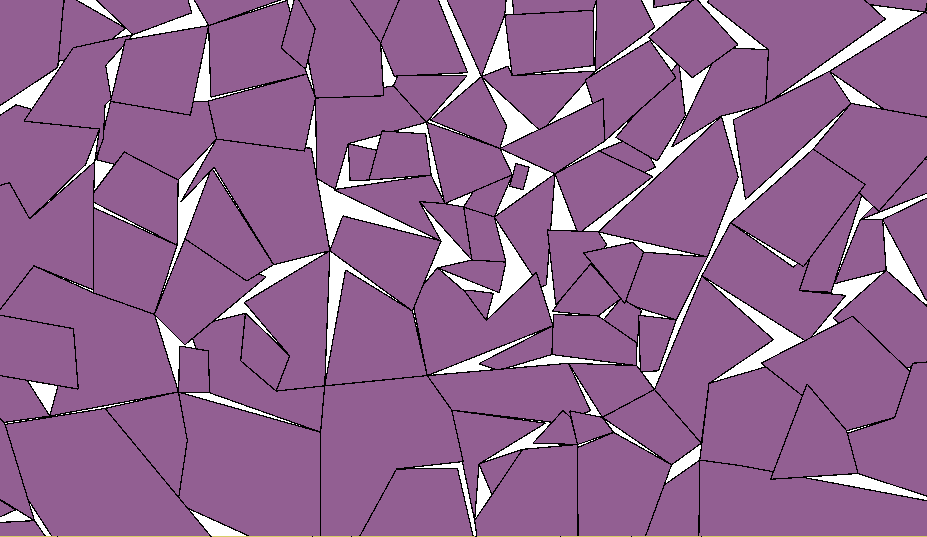
\includegraphics[width=0.90\textwidth]{pnro_simp500.png}
\caption{Alueet yleistettynä yksittäin ilman naapurialueiden huomioimista.}
\label{kuva2}
\end{center}
\end{figure}
\end{frame}

\begin{frame}[fragile=singleslide]\frametitle{Esimerkki 1: Topologinen yleistys (geom\_simp)}
\begin{figure}[h]
\begin{center}
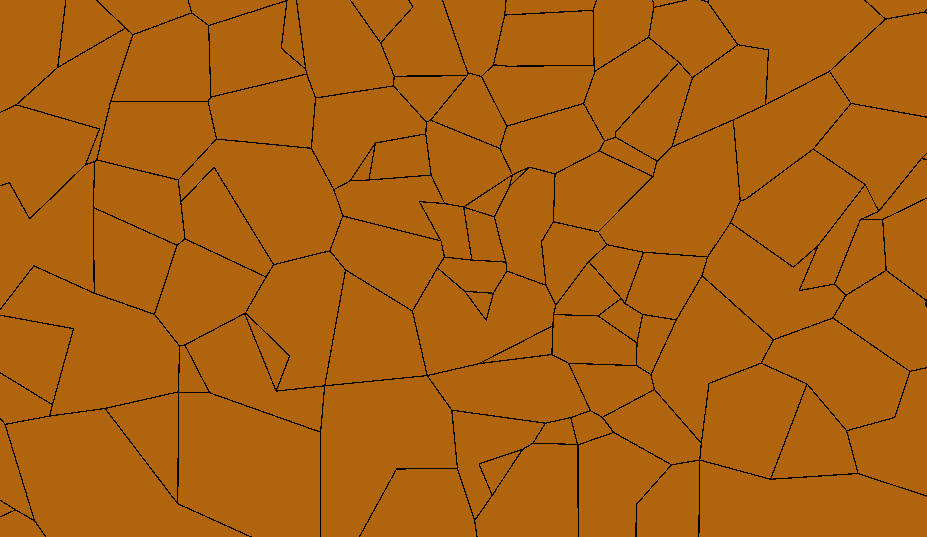
\includegraphics[width=0.90\textwidth]{pnro_toposimp500.png}
\caption{Alueet yleistettynä yhteisten rajaviivojen avulla (postgis\_topology)}
\label{kuva3}
\end{center}
\end{figure}
\end{frame}

\begin{frame}[fragile=singleslide]\frametitle{Esimerkki 2: Rekursio postinumeroalueilla}
\begin{verbatim}[fontsize=\footnotesize]
-- 00100 Postinumeroalueen naapureita
WITH RECURSIVE t(ogc_fid, the_geom, n, visited, cycle) AS (
     SELECT pno_meri.ogc_fid, pno_meri.wkb_geometry, 
            1, ARRAY[]::int[], false
     FROM statfi.pno_meri
     WHERE pno_meri.posti_alue = '00100'
   UNION ALL
     SELECT pno_meri.ogc_fid, pno_meri.wkb_geometry, 
            t.n + 1, t.visited || t.ogc_fid, t.ogc_fid = ANY(t.visited)
     FROM statfi.pno_meri, t
         WHERE t.the_geom && pno_meri.wkb_geometry
	   AND ST_Overlaps(ST_Boundary(t.the_geom), 
                           ST_Boundary(pno_meri.wkb_geometry))
	   AND t.ogc_fid != pno_meri.ogc_fid
	   AND NOT ARRAY[pno_meri.ogc_fid] <@ t.visited
	   AND t.n < 6
	   AND NOT cycle
)
SELECT DISTINCT n, ST_Transform(the_geom, 900913) FROM t;
\end{verbatim}
\end{frame}

\begin{frame}[fragile=singleslide]\frametitle{Esimerkki 3: KNNGIST-haku OSM-aineistolla}
  \begin{itemize}
  \item OSM-ainesto haettu maittain: http://download.geofabrik.de/
  \item Tietokantaan vienti: osm2pgsql
  \item Partitioitu maittain perintää käyttäen
  \item Luotu GIST-indeksi geometriakentälle "way" ja GIN-indeksi hstore-kentälle "tags"
  \item Aineiston koko:
\begin{verbatim}[fontsize=\footnotesize]
    
SELECT pg_size_pretty(
  sum(pg_total_relation_size(schemaname || '.' || tablename)))
FROM pg_tables WHERE tablename LIKE 'osm_%_point';
 pg_size_pretty 
----------------
 2601 MB
(1 row)
\end{verbatim}
  \end{itemize}
\end{frame}

\begin{frame}[fragile=singleslide]\frametitle{Esimerkki 3: KNNGIST-haku OSM-aineistolla}
\begin{verbatim}[fontsize=\footnotesize]
--
-- 100 lähintä pubia kursorin paikasta
--
SELECT way, ST_Distance(ST_SetSRID((::cp::)::geometry, 900913), way)
FROM osm.osm_point
WHERE amenity = 'pub'
ORDER BY osm_point.way <-> ST_SetSRID((::cp::)::geometry, 900913)
LIMIT 100;

--
-- Karaokella (?-operaattori hyödyntää tags-kentän GIN-indeksiä)
--
SELECT way, tags -> 'karaoke' AS karaoke, 
    ST_Distance(ST_SetSRID((::cp::)::geometry, 900913), way)
FROM osm.osm_point
WHERE amenity = 'pub'
  AND tags ? 'karaoke'
ORDER BY osm_point.way <-> ST_SetSRID((::cp::)::geometry, 900913);
\end{verbatim}
\end{frame}


\begin{frame}[fragile=singleslide]\frametitle{Mandelbrot-fraktaali}
\begin{verbatim}[fontsize=\tiny]
--
-- Mandelbrot SQL:llä
-- (vaatii Common Table Expression -tuen).
--
--  http://wiki.postgresql.org/wiki/Mandelbrot_set
--
WITH RECURSIVE x(i) AS (
    VALUES(0)
UNION ALL
    SELECT i + 1 FROM x WHERE i < 101
),
Z(Ix, Iy, Cx, Cy, X, Y, I) AS (
    SELECT Ix, Iy, X::float, Y::float, X::float, Y::float, 0
    FROM
        (SELECT -2.2 + 0.031 * i, i FROM x) AS xgen(x,ix)
    CROSS JOIN
        (SELECT -1.5 + 0.031 * i, i FROM x) AS ygen(y,iy)
    UNION ALL
    SELECT Ix, Iy, Cx, Cy, X * X - Y * Y + Cx AS X, Y * X * 2 + Cy, I + 1
    FROM Z
    WHERE X * X + Y * Y < 16.0
    AND I < 27
), Zt (Ix, Iy, I) AS (
    SELECT Ix, Iy, MAX(I) AS I
    FROM Z
    GROUP BY Iy, Ix
    ORDER BY Iy, Ix
)
SELECT ST_Translate(ST_Buffer(
                              ST_MakePoint(3000*Ix, 3000*Iy), 
                              20 + I*25),
	            -150000, 7100000, 0)
FROM Zt;
\end{verbatim}
\end{frame}

\begin{frame}[fragile=singleslide]\frametitle{Mandelbrot-fraktaali}
\begin{figure}[h]
\begin{center}
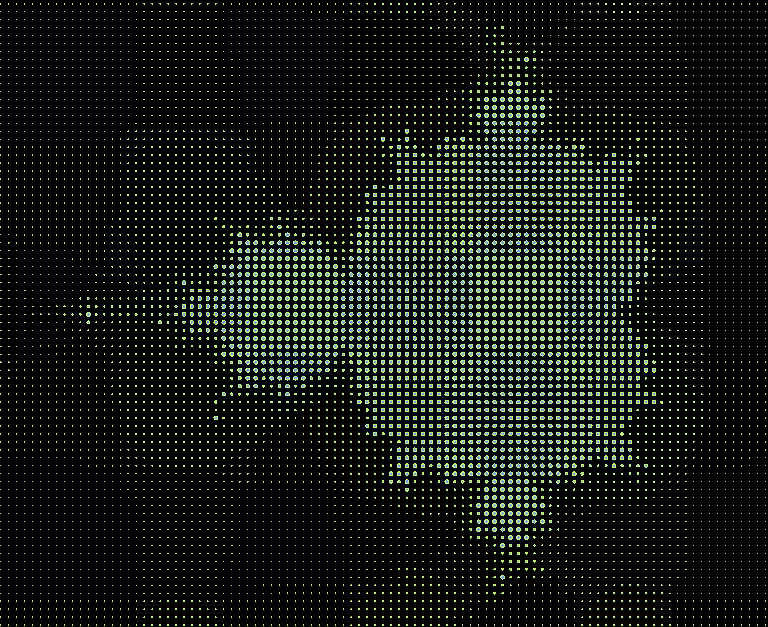
\includegraphics[width=0.90\textwidth]{mandelbrot.png}
\caption{Kyselyn tuottamat geometriat.}
\label{kuva4}
\end{center}
\end{figure}
\end{frame}

\end{document}
